\chapter{Backend-System}
\label{chp:backend}

Das Backend, entwickelt im Java Spring Framework, übernimmt die Verarbeitung der empfangenen Daten. Mithilfe von \emph{Kafka for Spring Framework} werden die Daten von Apache Kafka abgerufen und an das Backend übergeben. Danach werden die Daten in eine \emph{PostgreSQL} Datenbank persistiert, mittels dem \emph{Spring Data JDBC} Module von dem \emph{Spring Framework}. Damit die Daten auch verwendet werden können, werden sie über eine \emph{GraphQL} Schnittstelle zur Verfügung gestellt. In diesem Kapitel wird über die Lösungsansätze für Probleme, welche während der Implementierung im Prototyp aufgetreten sind, berichtet.


\section{Apache Kafka und Java Spring Framework}
\label{apacheKafkaImpl}

\emph{Apache Kafka} ist ein open-source \emph{Messaging System}, welches in dieser Arbeit für die entkoppelte Datenübertragung von der Siemens GNA Software zu dem Backend, eingesetzt wird. Kafka ist für die Anwendung in großen verteilten System konzeptioniert, welche sehr hohe Anforderungen an einer Reihe von Aspekten, wie zum Beispiel Ausfallsicherheit oder Skalierbarkeit haben. Dadurch wird Apache Kafka ein sehr mächtiges, aber auch komplexes Messaging System, welches in der Einrichtung und Verwendung sehr aufwendig sein kann. In diesem Kapitel wird beschrieben, wie durch die Nutzung der richtigen Techniken und Tools dieser Aufwand fast völlig eliminiert worden ist.

\subsection{Einrichtung von Apache Kafka}

Die Architektur von jeder Apache Kafka Installation besteht aus mindestens einer \emph{Zookeeper} Instanz und einer Kafka Instanz. Damit die Einrichtung stark vereinfacht wird, nutzt der Prototyp die Apache Kafka Distribution für \emph{Docker}, entwickelt von dem Unternehmen Confluent. 

Docker ist eine Open-Source-Plattform, die es Entwicklern ermöglicht, Anwendungen in sogenannten \emph{Containern} zu erstellen, zu verwalten und auszuführen. Container sind leichte, tragbare und isolierte Umgebungen, die alle notwendigen Abhängigkeiten enthalten, um eine Anwendung auszuführen, einschließlich des Betriebssystems, der Laufzeitumgebung, Bibliotheken und anderer Konfigurationen. Docker vereinfacht die Bereitstellung von Anwendungen, indem es eine konsistente Umgebung über verschiedene Systeme hinweg bereitstellt und eine schnellere Entwicklung und Bereitstellung ermöglicht. \cite{turnbull2014docker}

\emph{Docker Compose} ist ein Tool, das es ermöglicht, mehrere Docker-Container als eine einzige Anwendung zu definieren und zu verwalten. Mit Docker Compose können Entwickler eine YAML-Datei verwenden, um die Konfiguration mehrerer Container zu definieren, einschließlich ihrer Abhängigkeiten, Netzwerkeinstellungen und anderer Konfigurationsoptionen. Docker Compose erleichtert die Lokalisierung und Bereitstellung von komplexen Anwendungen, die aus mehreren miteinander verbundenen Containern bestehen, und ermöglicht eine einfache Wartung dieser Anwendungen.
\cite{turnbull2014docker}

Im Kontext des Prototyps ermöglicht Docker eine verlässliche Installation von Apache Kafka auf jeder Art von Umgebung, welche Docker selbst installiert haben. Dadurch können Sie diese Distribution von Kafka auf Linux, Windows oder auch macOS installieren, ohne befürchten zu müssen, dass Fehler durch diese unterschiedlichen Umgebungen entstehen. Docker Compose schafft die Komplexität, welche Apache Kafka durch seine verteilte und ausfallsichere Natur hat, in einer deklarativen Art zu minimieren. Diese Einfachheit kann in dem Quellcode \ref{lst:dockerComposeFileApacheKafka} erkannt werden, denn Zookeeper und Apache Kafka können in einer übersichtlichen Weise konfiguriert werden. Ein weiterer Vorteil ist, dass die ganze Konfiguration in einem einzigen File definiert ist, welches eine einfache Installation auf mehreren Systemen ermöglicht. 

\begin{lstlisting}[language={yaml},caption={Docker Compose File zur einfachen Einrichtung von Apache Kafka},captionpos=b,label={lst:dockerComposeFileApacheKafka}]
version: '3'
name: 'ndfa-backend'
services:
  zoo:
    image: confluentinc/cp-zookeeper:latest
    hostname: zoo
    ports:
      - "127.0.0.1:2181:2181"
    environment:
      ZOOKEEPER_CLIENT_PORT: 2181
      ZOOKEEPER_SERVER_ID: 1
      ZOOKEEPER_SERVERS: zoo:2888:3888

  kafka:
    image: confluentinc/cp-kafka:latest
    hostname: kafka
    ports:
      - "127.0.0.1:9092:9092"
      - "127.0.0.1:9999:9999"
    environment:
      KAFKA_ADVERTISED_LISTENERS: INTERNAL://kafka:19092,EXTERNAL://${DOCKER_HOST_IP:-127.0.0.1}:9092
      KAFKA_LISTENER_SECURITY_PROTOCOL_MAP: INTERNAL:PLAINTEXT,EXTERNAL:PLAINTEXT
      KAFKA_INTER_BROKER_LISTENER_NAME: INTERNAL
      KAFKA_ZOOKEEPER_CONNECT: "zoo:2181"
      KAFKA_BROKER_ID: 1
      KAFKA_LOG4J_LOGGERS: "kafka.controller=INFO,kafka.producer.async.DefaultEventHandler=INFO,state.change.logger=INFO"
      KAFKA_OFFSETS_TOPIC_REPLICATION_FACTOR: 1
      KAFKA_TRANSACTION_STATE_LOG_REPLICATION_FACTOR: 1
      KAFKA_TRANSACTION_STATE_LOG_MIN_ISR: 1
      KAFKA_JMX_PORT: 9999
      KAFKA_JMX_HOSTNAME: ${DOCKER_HOST_IP:-127.0.0.1}
      KAFKA_AUTHORIZER_CLASS_NAME: kafka.security.authorizer.AclAuthorizer
      KAFKA_ALLOW_EVERYONE_IF_NO_ACL_FOUND: "true"
    depends_on:
      - zoo
\end{lstlisting}

\subsection{Verwendung von Apache Kafka im Java Spring Framework}
\label{verwendungKafkaSpring}   
Um eine einfache und abstrakte Interaktion mit Apache Kafka zu ermöglichen, nutzt der Prototyp das \emph{Java Spring Framework} Modul \emph{Kafka for Spring Framework}. Damit kann eine nahtlose Integration von Kafka in das Spring Framework erfolgen und eine einfache Entwicklung von Systemen, welche mit dem Apache Kafka Messaging System funktionieren, möglich gemacht werden.

Konkret müssen zwei verschiedene Informationen über das Kafka-System zum Backend übertragen werden. Ein wichtiger Datensatz bilden die Informationen über die Modelobjekte, welche sich im Stromnetzwerk befinden. Modelobjekte sind Bestandteile des Netzes, wie beispielsweise ein Transformator, ein Verbindungskabel oder ein Energieerzeuger, diese werden in einer JSON-Repräsentation von der Siemens GNA Software zum Messaging-System geschickt. Ein Beispiel eines Modelobjekts ist im Quellcode \ref{lst:kafkaModelObjektJson} zu finden. Außerdem sollte man einen Blick auf das JSON-Property "linkedObjects" werfen, denn es beschreibt mithilfe der Modelobjekt-IDs die Verbindungen zu anderen Bestandteilen des Stromnetzmodelles, diese Information ist essenziell für den Aufbau des Graphen im Frontend. Solche JSON-Objekte werden bei der Installation des Prototyps in einer großen Menge zum Backend geschickt. Wird das Stromnetz später verändert, kann es in einer inkrementellen Weise beim Backend angepasst werden, denn wenn ein bestehendes Modelobjekt geändert werden muss, kann es einfach ersetzt werden. Um eine Löschung eines Objektes durchzuführen, muss einfach nur die Modelobjekt-ID alleine übertragen werden. 

\begin{lstlisting}[language={json},caption={Ein JSON-File, welches ein Modelobjekt im Stromnetzwerk beschreibt},captionpos=b,label={lst:kafkaModelObjektJson}]
{
  "guid": "9f447342-63fd-487a-8275-9da4b742258e",
  "name": "Dori_2",
  "className": "com.siemens.gna.internalModel.identifiedObjects.Node",
  "modelObjectType": "NODE",
  "container": "c8901795-ed4b-4768-8f5f-215429ec70aa",
  "linkedObjects": [
    "02f6ae6d-5d4c-4cfc-8e61-7a789f773cc0",
    "fadfedaa-ef18-47ad-92f2-56ae4584f59c",
    "b74d5d44-a972-4da1-a064-249a7ac75759"
  ]
}
\end{lstlisting}

Der zweite Teil der Daten, welche von der Siemens GNA Software dem Backend übermittelt werden, sind die Fehlerinformationen. Die Analyse von Fehlern im Stromnetz erfolgt periodisch und wenn ein Fehler gefunden wird, dann wird dieser dem Backend über Kafka geschickt. Diese Fehler werden auch als ein JSON-Objekt übertragen, wie beispielsweise im Quellcode \ref{lst:kafkaFindingJson}. Ein Fehler bezieht sich immer auf ein Objekt des Stromnetzmodelles, daher gibt es das JSON-Property "staticDataModelObjectGuid", welches den Verweis auf ein Objekt enthält. Eine besondere Bedeutung hat das Property "action", denn es kann zwei verschieden Aktionen auslösen. Wenn dieses Feld auf "ADD" gesetzt ist, dann wird ein neuer Fehler, welcher sich im Property "finding" befindet eingefügt. Falls dieses Feld aber auf "TRUNCATE" gesetzt ist, dann werden alle bisher gespeicherten Fehler in der Datenbank gelöscht. 

\begin{lstlisting}[language={json},caption={Die Fehlerinformationen über einen gefundenen Fehler im Netz},captionpos=b,label={lst:kafkaFindingJson}]
{
  "action": "ADD",
  "finding": {
    "staticDataModelObjectGuid": "d704c1d0-5c31-4cee-a016-a5381fd4c868",
    "powerSystemResourceGuid": "d704c1d0-5c31-4cee-a016-a5381fd4c868",
    "severity": "CRITICAL",
    "category": "semantic",
    "rawMessage": "Overhead Line has wrong r/x ratio. Should be < 0.5 and is %s",
    "messageParameters": [
      "1,45"
    ],
    "assambledMessage": "Overhead Line has wrong r/x ratio. Should be < 0.5 and is 1,45"
  }
}
\end{lstlisting}


Die vollständige Konfiguration von der Backend-Applikation bezüglich Kafka kann in der globalen Konfigurationsdatei von Spring erfolgen, das ist sehr vorteilhaft, weil so leicht die Übersicht behalten werden kann. In dem Quellcode \ref{lst:kafkaAppsettings} ist ein Auszug dieser Datei, welcher sich auf Kafka fokussiert. 

\begin{lstlisting}[language={yaml},caption={Auszug aus der Konfigurationsdatei für Spring },captionpos=b,label={lst:kafkaAppsettings}]
  kafka:
    bootstrap-servers: "${KAFKA_BOOTSTRAP_SERVERS:localhost:9092}"
    consumer:
      auto-offset-reset: earliest
      group-id: "ndfa"
      key-deserializer: org.apache.kafka.common.serialization.StringDeserializer
      value-deserializer: org.springframework.kafka.support.serializer.JsonDeserializer
      max-poll-records: 10000
\end{lstlisting}

Ein weiterer Aspekt der Konfiguration, welcher nicht in der globalen Konfigurationsdatei passiert, ist die Definition von \emph{Topics}, das sind Kanäle, auf denen Nachrichten geschickt und von \emph{Consumer} konsumiert werden können. In dem Code \ref{lst:kafkaTopicsSpring} kann leicht erkannt werden, wie einfach die Erstellung von Topics mit der Hilfe von Kafka for Spring Framework ist. Im Falle des Prototyps sind zwei Kafka-Themen in Verwendung. Das "Findings"-Topic ist zuständig für die Übertragung der gefundenen Fehler und das zweite wird für die Übermittlung des Stromnetzmodells benötigt.

\begin{lstlisting}[language={python},caption={Definiton eines Topics mithilfe von Kafka for Spring Framework },captionpos=b,label={lst:kafkaTopicsSpring}]
@Bean
public KafkaAdmin.NewTopics createTopics() {
    return new KafkaAdmin.NewTopics(

            TopicBuilder.name("model_objects")
                    .build(),
            TopicBuilder.name("findings")
                    .build()
    );
}
\end{lstlisting}

Ein sehr wichtiger Teil bezüglich der Interaktion mit Apache Kafka, ist die Erstellung von Consumer, denn sie können die Nachrichten von Topics auslesen. Durch die Unterstützung des Spring Modul kann mit einer Leichtigkeit, Consumer erstellt werden. Außerdem können spezielle Konfigurationen auch umgesetzt werden, beispielsweise, wie es im Code \ref{lst:kafkaConsumerSpring} zu erkennen ist, kann leicht \emph{Batch-Processing} beim  Auslesen umgesetzt werden. Des Weitern kann auch eine gleichzeitige Auslesung von Topics oder die Konvertierung von dem \emph{Message Body} in Java Klassen eingestellt werden. Im Prototyp hat das "Findings"-Topic und das "ModelObject"-Topic beide Batch-Processing aktiviert, damit eine schnelle Verarbeitung der Daten ermöglicht wird. Das Kafka-Thema, welches für die Modellobjekte des Stromnetzes zuständig ist, kann sogar mit mehreren Threads das Topic parallel auslesen, da die Reihenfolge der Nachrichten keine Rolle spielt.

\begin{lstlisting}[language={java},caption={Definiton eines Consumers mithilfe von Kafka for Spring Framework },captionpos=b,label={lst:kafkaConsumerSpring}]
@KafkaListener(topics = "model_objects", batch = "true", concurrency = "3",
        properties = { "spring.json.value.default.type=com.siemens.backend.model.gna.GnaModelObject" }
)
public void processMessage(List<GnaModelObject> content) throws SQLException {
    logger.debug("received %s GnaModelObjects on topic model_objects".formatted(content.size()));
   modelObjectsService.insertAndDeleteGnaModelObjects(content);
}
\end{lstlisting}

Es wurde in den vorherigen Absätzen bestätigt, dass die Verwendung von Kafka for Spring Framework, eine einfache Integration von Apache Kafka in den Java Code schaffen kann. Durch die starke Abstrahierung können sogar Entwickler, welche sich mit dem Messaging-System nicht so gut auskennen, trotzdem damit programmieren.
\section{PostgreSQL}
\label{postgresImpl}

\emph{PostgreSQL} ist eine objektrelationale Datenbank, welche für die Persistierung der Daten, die über Apache Kafka erhalten worden sind, zuständig ist. Jedoch beschreiben diese Daten ein Stromnetzwerk, welches von Natur aus einer Graphenstruktur ähnelt. Graph-Daten sind immer stark vernetzt und somit problematisch für die Speicherung in relationale Datenbanken. In diesem Kapitel wird genauer diese Problematik beschrieben und der gewählten Lösungsweg vorgestellt. 

\subsection{Problematik der Speicherung von Graph-Daten in einer relationalen Datenbank}
Eine relationale Datenbank organisiert Daten in Tabellen, wobei jede Tabelle eine Sammlung von Zeilen und Spalten darstellt. Jede Zeile in einer Tabelle entspricht einem Datensatz, während jede Spalte ein Attribut oder eine Eigenschaft dieses Datensatzes darstellt. Die Struktur des relationalen Datenbankmodells wird durch eine Reihe von Regeln definiert, die sicherstellen, dass die Daten konsistent sind. Ein einfaches Beispiel wäre die Zuordnung von mehrere Schüler zu einem Lehrer. Dafür muss eine Lehrertabelle und Schülertabelle erstellt werden und zusätzlich in der Schülertabelle eine weitere Spalte hinzugefügt werden, welche die IDs der Lehrer beinhaltet, um eine Verbindung aufzubauen. Diese Spalte wird auch die Fremdschlüsselspalte genannt, denn es wird ein fremder Schlüssel (ID von Lehrer), also eine ID, welche nicht von demselben Datensatz herkommt, in die Zeile eingefügt. 

Ein offensichtliches Problem bei dieser Art Verbindungen aufzubauen ist, wenn Sie eine N:M Relation umsetzen möchten. Solch eine Relation in den Kontext des Beispiels würde bedeuten, dass Schüler mit mehreren Lehrern und Lehrer mit mehreren Schülern in Verbindung stehen. Jedoch ist es nicht möglich, diesen Fall nur mit einer Fremdschlüsselspalte umzusetzen, denn dafür müssten Sie mehrere IDs in dieser Spalte einfügen, was aber das grundsätzliche Konzept der Atomarität der Spalten verletzt. Um diese Relation dennoch umzusetzen, muss eine weitere Tabelle hinzugefügt werden, welche in jeder Zeile eine Verbindung zwischen einem Lehrer und einem Schüler definiert. Diese weitere Tabelle fügt einen weiteren Schritt für der Auflösung der Beziehungen hinzu, was eine schlechtere Abfrageperformance zur Folge hat. 

Ein weiteres Problem zeigt sich bei der Einfügung der Daten in die Tabellenstruktur. Denn normalerweise wird eine Fremdschlüsselspalte durch eine Regel geschützt, welche nur Schlüssel von einer bestimmten Tabelle erlaubt. Will jedoch eine Zeile hinzugefügt werden, welche einen noch nicht eingefügten Datensatz referenziert, ist das nicht möglich und der Datensatz muss zwischengespeichert werden. In dem Fall dieser Arbeit ist dieses Problem bedeutend, da die Daten in kleine Stücke über Apache Kafka erhalten werden und deren Reihenfolge nicht definiert wurde. Außerdem ist das Berechnen der richtigen Reihenfolge von großem Aufwand, insbesondere wenn Sie die Größe der Daten, welche das Stromnetzwerk beschreiben, bedenken. Das Problem prägt sich aus durch eine überaus lange Zeit, welche benötigt wird, um die Daten vollständig einzufügen. 

Damit diese zwei Probleme gelöst werden konnten, ist ein Lösungsansatz herausgearbeitet worden, welcher in dem folgenden Kapitel erläutert wird.

\subsection{Lösungsansatz für effiziente Speicherung von Graph-Daten}

Dieser Lösungsansatz verfolgt zwei verschiedene Konzepte, um die Problematik zu lösen. Einerseits, die Vereinfachung der Tabellenstruktur und andererseits die Auflösung aller Regeln bezüglich der Fremdschlüssel in Tabellen. 

Anstatt eine komplexe Struktur von Tabellen aufzubauen, wird im Prototypen eine einfache Struktur angestrebt. Jedoch sollte auch angemerkt werden, dass Daten durch einen komplexen Aufbau der Tabellen leichter konsistent gehalten werden können. Aber im Kontext dieser Arbeit wird dieser Vorteil zum Nachteil, weil das Datenmodell muss in der Lage sein, jegliche Fehler des Stromnetzmodelles darzustellen. Die finale Struktur der Tabellen kann in der Abbildung \ref{fig:Tabellenstruktur} betrachtet werden. Es wird auf jede überflüssige Tabelle verzichtet und somit können performante Abfragen erreicht werden. 

In der Darstellung kann auch erkannt werden, dass es keine Verbindungen zwischen den Tabellen gibt, welche eine Relation andeuten. Aber tatsächlich gibt es für jedes Finding (Fehler in Netzmodell) ein oder mehrere Modelobjekte, welche die eigentlichen Objekte des Stromnetzes beschreiben, beispielsweise könnte ein Modelobjekt ein Transformator oder eine Hochspannungsleitung darstellen. Zusätzlich sind natürlich die Objekte des Stromnetzes miteinander verbunden, dafür wird die \emph{Connections} Tabelle benötigt, denn sie stellt jede Verbindung mit einer Zeile dar. Diese Verbindungen werden nicht angezeigt, weil sie durch kein Regelwerk definiert worden sind. Durch den Verzicht auf diese Regeln können die Datensätze direkt in die Datenbank eingefügt werden und die Zeit für die Befüllung der Datenbank nach Änderung des Stromnetzmodelles kann minimiert werden.   

\begin{figure}[t!]
    \centering
    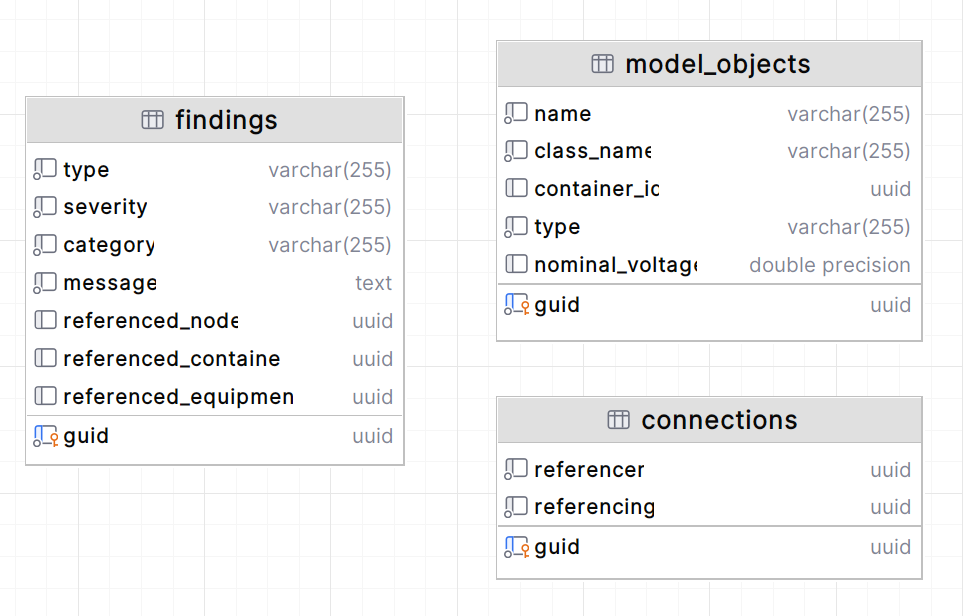
\includegraphics[width=0.9\textwidth]{content/img/Empire/Backend/tabellenstruktur.png}
    \caption{Tabellenstruktur des Prototyps}
    \label{fig:Tabellenstruktur}
\end{figure}
\FloatBarrier

\hspace{5em}